\section{Alzheimer's disease}

% Severity of Alzheimer's Disease.
Alzheimer's Disease (AD) is characterized by a progressive degeneration of the brain and cognitive functions \cite{Lane2018}. In the literature, diagnosis of patients is usually divided in three stages \cite{Brookmeyer2007}, although other classifications have been recently proposed:

\begin{enumerate}\itemsep5pt
\item Healthy Control or Cognitively Normal (CN), when the patient shows neither signs of the disease nor cognitive problems.
\item Mild Cognitive Impairment (MCI), when the patient shows signs of cognitive impairment. It can be divided into two substages: early MCI and late MCI, differentiating between patients by their degree of cognitive impairment.
\item AD, when the patient is considered to have completely progressed into full-blown dementia.
\end{enumerate}

Figure \ref{appendix:figAD} shows an MRI axial view of two different patients: one healthy control and the other with AD. We can appreciate the effects of the disease directly on the reduction of cortical thickness, among other visual and physical cues \cite{Schmidt1992}. \\

\begin{figure}[htbp]
  \centering
%  \includegraphics[width=0.75\textwidth]{figures/mri_scans.png}
  \caption{Axial view of MRI scan for AD (left) and CN (right) patients. Images from ADNI dataset, registered to a common template.}
  \label{appendix:figAD}
\end{figure}

\subsection{AD markers} 

To determine the stage of the disease, various markers describing key pathophysiological processess of AD have been proposed over the years. Markers of the brain provide information for the study of the disease and its screening. AD is characterized by protein amyloid-beta (A$\beta$) deposition in the brain \cite{Rissman2012}, tau injury, and structural neurodegeneration \cite{Jack2013}. Those three indicators precede cognitive impairment, leading to death. For the measurement of these indicators, different markers have been proposed:

\begin{enumerate}\itemsep5pt
\item Brain A$\beta$ deposition in the brain can be detected both in positron emission tomography (PET) imaging \cite{Clark2011}, and in cerebrospinal fluid (CSF) \cite{Andreasen1999}.
\item Tau injury and dysfunction caused by tau and p-tau plaques, found in tau-PET imaging and CSF \cite{Andreasen1999,Blennow2010}.
\item Neurodegeneration provoked by tau injury. It can be observed in structural magnetic resonance imaging (MRI) \cite{Weiner2005} and in fludeoxyglucose (FDG)-PET imaging \cite{Chetelat2003}.
\item Memory and cognition, measured by cognitive tests.
\end{enumerate}

%% Screening
The main screening tool for clinical assessment of AD is the clinical interview between the patient and the doctor, where the severity of the cognitive problems of the patient can be assessed, followed by a cognitive physical examination to capture the aforementioned markers and assess the presence of the disease \cite{Lane2018}. \\

Apart from the aforementioned markers and imaging techniques, resting-state electroencephalography (EEG) signals have also been proposed for AD assessment \cite{Al-Qazzaz2014,Bhat2015}. However, they are not as widely used as image-based examination, as EEG cannot be used to observe specific processes in the brain and they only show changes in brain activity, which could be caused by other pathologies. A review on EEG methods for AD can be found in \cite{Houmani2018}.

\subsection{Longitudinal marker dynamics and disease model}

The previous markers can be studied and modelled longitudinally. Modelling their trajectories and progression can give us more insight on how they change and interact. For example, longitudinal data analysis on MRI allows us to calculate the rate of change of specific brain structures, such as the dynamics of cortical and hippocampal atrophy. \\

A widely accepted progression model of AD was proposed by \cite{Jack2010}. Their model is based on marker evolution, where each marker progresses from normal values to abnormal values differently. The order of the markers is the presented above: A$\beta$ deposition, followed by tau injury, neurodegeneration and cognition. Empirical data and experiments reviewed in \cite{Jack2013} confirm the validity of the model, although other data-driven works do not fully agree with it \cite{Iturria-Medina2016}. Analyzing those markers longitudinally allows us to study both the individual and whole population rate of change, and improve AD progression modelling. \\

\subsection{Studies and initiatives} 
\label{biomarkers:studies}
%% Explain about studies that focus on longitudinal data. and about the challenges that promote the use of longitudinal data for progression of the disease.

There has been a remarkable number of initiatives to promote using longitudinal data on AD modelling. Availability of patients' longitudinal data is key to study the progression of the disease. \cite{Lawrence2017} presented a review of available longitudinal AD biomarker datasets, finding that more efforts are needed to increase the follow-up duration, increase the population sizes and standardize the acquisition methods. One of the largest studies is the Alzheimer's Disease Neuroimaging Initiative (ADNI) \cite{Mueller2005}, a multimodal, ongoing longitudinal study with hundreds of enrolled subjects, gathering imaging data, cognitive scores, blood and CSF markers. To unify and share the available data, the Alzheimer's Association has created The Global Alzheimer’s Association Interactive Network (GAAIN) \footnote{\url{http://www.gaain.org}} to share data between independent studies and build collaborations to create and explore large, heterogeneous cohorts. \\

% ADD MIRIAD Challenge
Initiatives to stimulate research on the field have also been proposed, such as the MIRIAD challenge \cite{miriad}, The Alzheimer's Disease Prediction Of Longitudinal Evolution (TADPOLE) Challenge\footnote{\url{https://tadpole.grand-challenge.org}} or Quantitative Templates for the Progression of Alzheimer’s disease (QT-PAD)\footnote{\url{http://www.pi4cs.org/qt-pad-challenge}}. These challenges define a fixed subset of available data, making it easier to compare results, share methods and ensure reproducibility. \\


\subsection{Biological definition of AD}
A new unified research framework for a biological definition of the disease was recently published by the National Institute on Aging and the Alzheimer's Association \cite{Jack2018}. This approach defines AD as a biological construct based on markers, rather than clinical symptoms of the disease such as cognitive impairments. The framework is flexible enough for the introduction of additional markers, if needed. \\

The framework groups markers in three categories: A$\beta$ deposition, pathologic tau, and neurodegeneration. This is represented as the AT(N) system, where each category can be binarized using a cut point into normal/abnormal (-/+). For each category:

\begin{itemize}
    \item \textbf{A:} A$\beta$ markers determine if a patient is in the Alzheimer's continuum, showing pathological changes but still not presenting the disease.
    \item \textbf{T:} tau deposition markers indicate whether a patient who is in the Alzheimer's continuum has the disease.
    \item \textbf{(N):} Neurodegeneration markers show structural changes in the brain that can be product of AD, but are not specific to the disease (and thus is placed in parenthese).
\end{itemize}

% Review of existing works and if there is anything longitudinal
The flexibility of the framework allows working with missing biomarker values, which is a valuable trait for a longitudinal study. We found no work (within the scope of this review) using this new biological definition on AD. The reasons could be the recentness of the framework's publication, and the need for multimodal data in a longitudinal setting, which is not as available as single modality MRI. However, we expect future studies to use this framework, as it offers clear advantages for longitudinal analysis: for example, being able to directly compare different stages of progression between patients, or extend the framework with markers that capture longitudinal progression.

\subsection{Challenges in longitudinal data}

Longitudinal data are composed of sequential data acquisitions for subjects over a period of time. This contrasts with cross-sectional studies, which focus on single acquisitions per subject. Here, we describe the main characteristics and analysis challenges that arise while dealing with longitudinal data. In Section \ref{sec:missing} we outline strategies to overcome some of them.  \\

Two sources of variability can be defined for a longitudinal study in a cohort of subjects: the inter-subject variability, i.e., the differences between observations of different subjects, and the intra-subject variability, i.e., the differences between observations of a same subject, which tend to be highly correlated compared to the former. Those two sources of variation give valuable information about the progression of the disease between- and within- subjects. In cross-sectional studies, those two variabilities are non-separable: given two samples of different subjects, it is not possible to know to what extent their variation is due to inter-subject variability or to the different stages of the disease. Adding longitudinal samples for each subject allows us to distinguish between those two variabilities, improving our understanding of the disease \cite{Fitzmaurice2008}. \\

\begin{figure}[htbp]
  \centering
  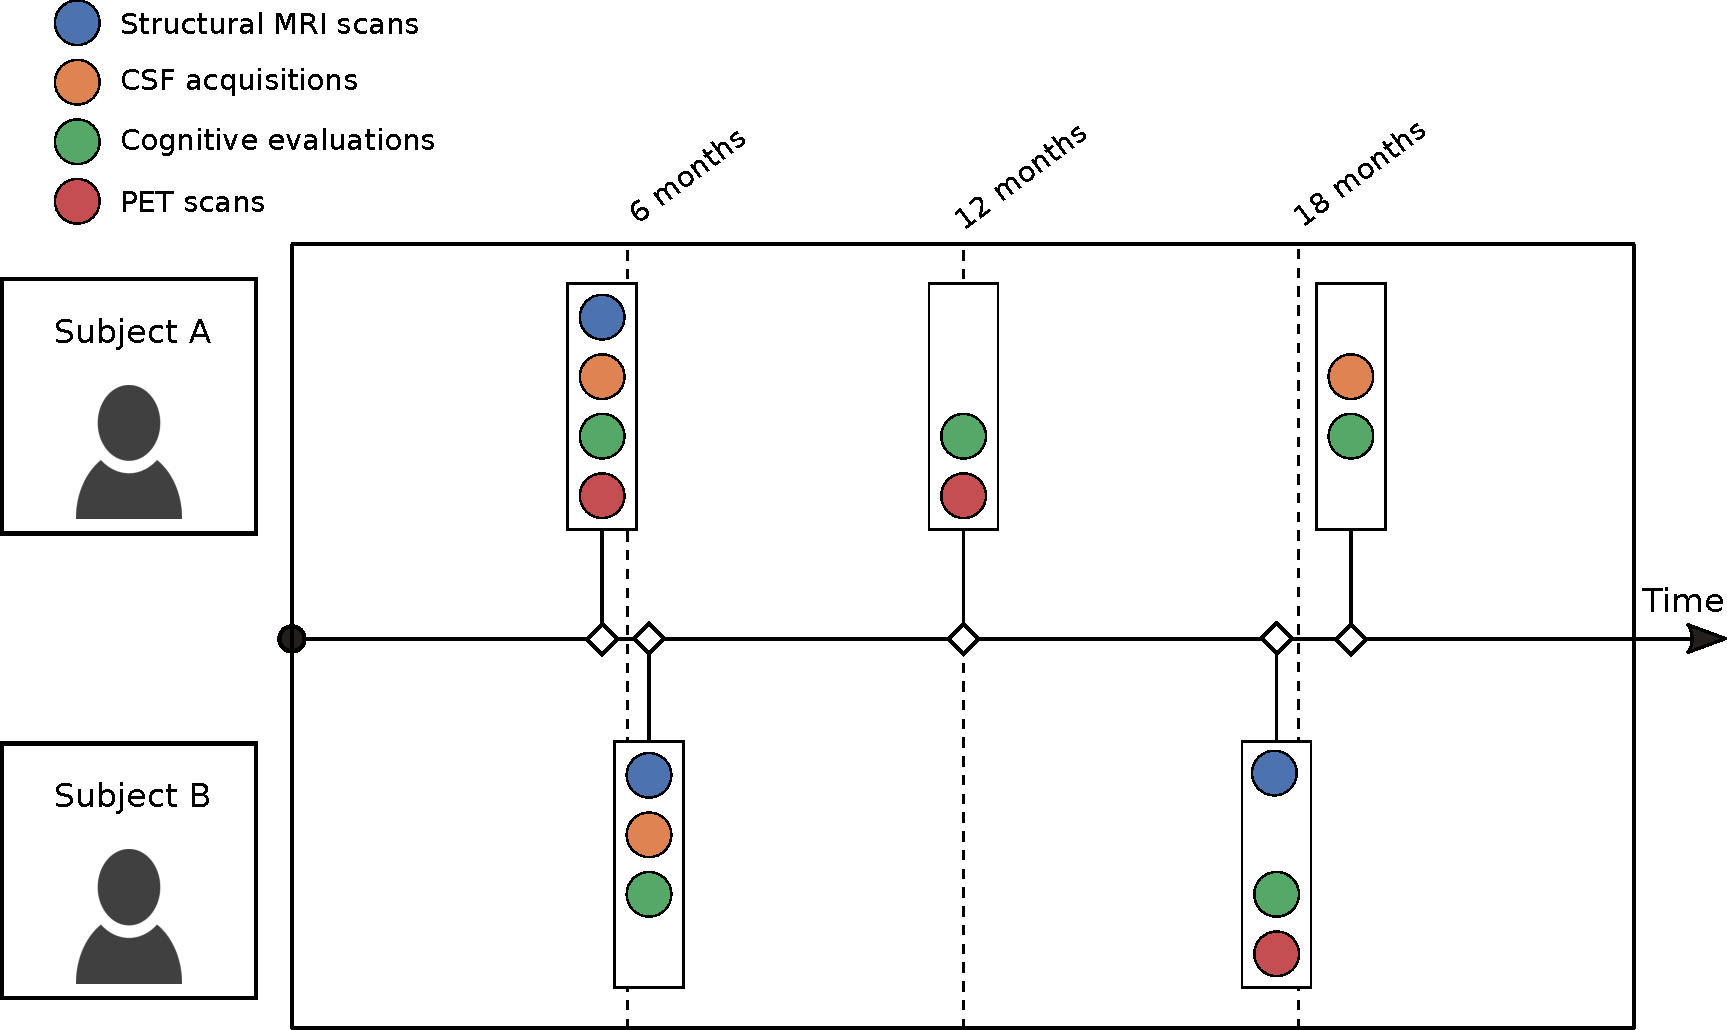
\includegraphics[width=1.0\textwidth]{figures/introduction/Fig2.pdf}
  \caption{Longitudinal representation of data acquisitions for two patients.}
  \label{long}
\end{figure}

Figure \ref{long} shows an example of a longitudinal study for two subjects, with multiple data modalities, over a fixed span of time. It illustrates some of the challenges that can appear in a longitudinal, multimodal data study: \\

% The figure should include these various points
\begin{enumerate}\itemsep5pt
\item Each subject can have a different number of acquisitions, leading to an unbalanced data problem. In the figure, Patient B missed the 12th month acquisition for some reasons.
\item There can be missing data due to missing acquisitions from some modalities. In the figure, only patient A at the 6-months follow-up has all the acquisitions. 
\item Data are not necessarily acquired at the same time point for the different subjects.
\item Time spacing between follow-ups can be variable, even within a single subject.
\end{enumerate}

Another problem, not shown in the figure, is that different patients can be at different stages of the disease at a given time point. Reference time to measure progression remains an open issue in the field \cite{Ashford2001}.  \\

Protocols of data acquisition try to palliate these problems, but in a clinical setting, this is very difficult to achieve: sometimes patients miss their scheduled screening session and data cannot be gathered. Other patients might drop out from the study for a variety of reasons, such as disease severity or moving out of the city/country, and in other cases, data of a given time point could need to be discarded because of quality problems. For these reasons, most of the available longitudinal data is unbalanced. \\

All studies should define their policy on this issue, either by selecting only subjects with no missing data in their studies, or by defining a method to handle the problem. Popular methods for missing data in longitudinal studies are detailed in \cite{Ibrahim}. \\

\section{Machine learning for medical data}



\section{Contributions}


\subsection{Outline of the thesis}

